 \documentclass[xcolor=dvipsnames,table]{beamer}
%o
%e

\usepackage{latexsym}
\usepackage [ansinew]{inputenc}
\usepackage[brazil]{babel}
\usepackage{amssymb} %Este e o AMS paquete
\usepackage{amsmath}
\usepackage{stmaryrd}
\usepackage{fancybox}
\usepackage{datetime}
\usepackage[inline]{enumitem}


\usepackage[T1]{fontenc}

%\usepackage{beamerthemesplit}
\usepackage{graphicx}
\usepackage{graphics}
\usepackage{url}
\usepackage{algorithmic}
\usepackage{algorithm}
\usepackage{acronym}
\usepackage{array}

\newtheorem{definicao}{Definio}
\newcommand{\tab}{\hspace*{2em}}

\mode<presentation>
{
  %\definecolor{colortexto}{RGB}{153,100,0}
  \definecolor{colortexto}{RGB}{0,0,0}
  
% \setbeamersize{sidebar width left=0.5cm}
  \setbeamertemplate{background canvas}[vertical shading][ bottom=white!10,top=white!10]
%   \setbeamercolor{title}{fg=colortitulo!80!black,bg=blue!20!white}
%   \setbeamercolor{title}{bg=colortitulo!20!black}
%   \setbeamercolor{background canvas}{bg=colortitulo}
%   \setbeamercolor{frametitle}{fg=red}

  \setbeamercolor{normal text}{fg=colortexto} 

  \usetheme{Warsaw}
  %\logo{\includegraphics[width=2cm]{Images/ratonfuerte.jpg}}


%   \usefonttheme[onlysmall]{structurebold}
%   \usecolortheme{seahorse}
%  \usecolortheme[named={YellowOrange}]{structure}
%   \usecolortheme[named={Blue}]{structure}
%   \usecolortheme{crane}
%   \useoutertheme{default}
}

\title{Linguagens N�o-regulares} 

\author{
  Esdras Lins Bispo Jr. \\ \url{bispojr@ufg.br}
}
 \institute{
  Linguagens Formais e Aut�matos \\Bacharelado em Ci�ncia da Computa��o}
\date{\textbf{02 de outubro de 2019} }

\logo{
\includegraphics[width=1cm]{images/ufjLogo.png}}

\begin{document}

	\begin{frame}
		\titlepage
	\end{frame}

	\AtBeginSection{
		\begin{frame}{Sum�rio}%[allowframebreaks]{Sum�rio}
    		\tableofcontents[currentsection]
    		%\tableofcontents[currentsection, hideothersubsections]
		\end{frame}
	}

	\begin{frame}{Plano de Aula}
		\tableofcontents
		%\tableofcontents[hideallsubsections]
	\end{frame}	
	
	\section{Instru��o pelos Colegas}
	
	\begin{frame}{Quest�o 057}	
		\begin{block}{[Q057]}
			O lema do bombeamento � utilizado para provar a n�o-regularidade de linguagens atrav�s da t�cnica de demonstra��o...
		\end{block}
		
		\begin{enumerate}[label=(\Alph*)]
			\item direta
			\item por indu��o
			\item por absurdo
			\item por constru��o
		\end{enumerate}
	\end{frame}
	
	\begin{frame}{Quest�o 058}	
		\begin{block}{[Q058]}
			\begin{columns}
				\begin{column}{0.05\textwidth}\end{column}
				\begin{column}{0.45\textwidth}
					A cadeia $0^p1^p$ pode ser usada para provar a n�o-regularidade da linguagem $A=\{0^n1^n$ | $n \geq 0 \}$, sendo $p$ o comprimento do bombeamento. Sobre esta cadeia e o lema do bombeamento, � \underline{incorreto} afirmar que...
				\end{column}
				\begin{column}{0.45\textwidth}
					\begin{center}
						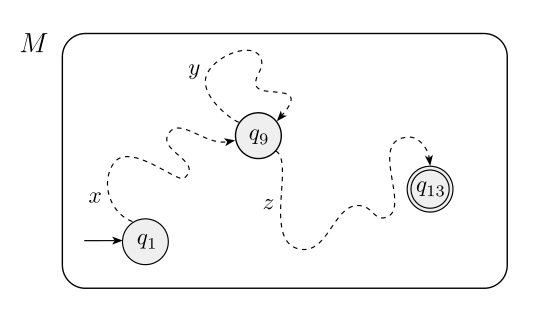
\includegraphics[width=1.0\textwidth]{images/xyz}
					\end{center}
				\end{column}
				\begin{column}{0.05\textwidth}\end{column}
			\end{columns}
		\end{block}
		
		\begin{enumerate}[label=(\Alph*)]
			\item $x$ pode ser igual a $\epsilon$.
			\item $y$ cont�m apenas 0s.
			\item $xyyz \not\in A$
			\item $z$ cont�m apenas 1s.
		\end{enumerate}
	\end{frame}

	\begin{frame}{Quest�o 059}	
		\begin{block}{[Q059]}
			A cadeia $0^p1^p$ pode ser usada para provar a n�o-regularidade da linguagem $A=\{\omega$ | $\omega$ tem n�mero igual de 0s e 1s $\}$, sendo $p$ o comprimento do bombeamento. Sobre esta cadeia e o lema do bombeamento, � \underline{incorreto} afirmar que...
		\end{block}
		
		\begin{enumerate}[label=(\Alph*)]
			\item $y$ pode ser igual a $\epsilon$.
			\item $y$ cont�m apenas 0s.
			\item $xz \not\in A$
			\item $z$ pode conter apenas 1s.
		\end{enumerate}
	\end{frame}

	\begin{frame}{Quest�o 060}	
		\begin{block}{[Q060]}
			A cadeia $0^p10^p1$ pode ser usada para provar a n�o-regularidade da linguagem $F=\{\omega\omega$ | $\omega \in \{0,1\}^*$ $\}$ , sendo $p$ o comprimento do bombeamento. Sobre esta cadeia e o lema do bombeamento, � \underline{incorreto} afirmar que...
		\end{block}
		
		\begin{enumerate}[label=(\Alph*)]
			\item $x$ pode ser igual a $\epsilon$.
			\item $y$ pode conter algum s�mbolo 1.
			\item $xyz \in A$
			\item $z$ cont�m algum s�mbolo 1.
		\end{enumerate}
	\end{frame}

	\begin{frame}{Quest�o 061}	
		\begin{block}{[Q061]}
			A cadeia $0^{p+1}1^p$ pode ser usada para provar a n�o-regularidade da linguagem $E=\{0^i1^j$ | $i>j$ $\}$ , sendo $p$ o comprimento do bombeamento. Sobre esta cadeia e o lema do bombeamento, � \underline{incorreto} afirmar que...
		\end{block}
		
		\begin{enumerate}[label=(\Alph*)]
			\item $x$ n�o pode conter algum s�mbolo 1.
			\item $y$ s� cont�m s�mbolos 0s.
			\item $xz \in A$
			\item $z$ cont�m algum s�mbolo 1.
		\end{enumerate}
	\end{frame}
	
	\begin{frame}
		\titlepage
	\end{frame}
	
\end{document}